\documentclass[t]{beamer}
\usefonttheme{serif}

\usepackage{amsmath,amsthm,amssymb,amsfonts,amscd,mathrsfs,amsxtra,multirow,kotex,mathtools,gensymb,textcomp,lipsum,tikz,verbatim,color,soul,courier,mdframed,xcolor}
\usepackage[normalem]{ulem}
\usetikzlibrary{calc,matrix,arrows,chains,positioning,scopes}
\usepackage{pdfpages}

\theoremstyle{plain}
\newtheorem{thm}{Theorem}[section]
\newtheorem{prop}[thm]{Proposition}

\theoremstyle{definition}
\newtheorem{defn}[thm]{Definition}
\newtheorem{exmp}[thm]{Example}
\newtheorem{excs}[thm]{Exercise}
\newtheorem{rem}[thm]{Remark}
\newtheorem{prob}[thm]{Problem}

\newcommand \tr[1]{\textcolor{red}{#1}}
\newcommand{\tikzmark}[1]{\tikz[overlay,remember picture] \node (#1) {};}
\newcommand{\varep}{\varepsilon}
\newcommand{\DrawBox}[1][]{%
    \tikz[overlay,remember picture]{
    \draw[red,#1]
      ($(left)+(-0.2em,0.9em)$) rectangle
      ($(right)+(0.2em,-0.3em)$);}
}

\newcommand{\tikzmarkk}[2]{
    \tikz[overlay,remember picture,baseline] 
    \node[anchor=base] (#1) {$#2$};
}
\newcommand*\circled[1]{\tikz[baseline=(char.base)]{
            \node[shape=circle,draw,inner sep=2pt] (char) {#1};}}

\tikzset{join/.code=\tikzset{after node path={%
\ifx\tikzchainprevious\pgfutil@empty\else(\tikzchainprevious)%
edge[every join]#1(\tikzchaincurrent)\fi}}}

\tikzset{>=stealth',every on chain/.append style={join},
         every join/.style={->}}
\tikzstyle{labeled}=[execute at begin node=$\scriptstyle,
   execute at end node=$]


\addtobeamertemplate{navigation symbols}{}{%
    \usebeamerfont{footline}%
    \usebeamercolor[fg]{footline}%
    \hspace{1em}%
    \raisebox{2pt}[0pt][0pt]{\insertframenumber/\inserttotalframenumber}
}
\setbeamercolor{footline}{fg=blue}
\setbeamerfont{footline}{series=\bfseries}
\title[]{SE102:Multivariable Calculus}

\author[]{Hyosang Kang\inst{1}}

\institute[]{\inst{1}Division of Mathematics\\ School of Interdisciplinary Studies\\ DGIST}

\date[]{Lecture 02\\
Continuity and Differentiability}

\begin{document}

\begin{frame}
\titlepage
\end{frame}

\begin{frame}
\begin{defn}
	The \textbf{polar coordinate} is a system of coordinate system
	which describes the Cartesian coordinate $P=(x,y)$
	as $(r,\theta)$ where $r$ is the length of
	$\overline{OP}$ and $\theta$ is the angle between 
	$\overline{OP}$ and positive $x$-axis.
\end{defn}
\begin{exmp}
	The vector $\vec r$ and $\vec\theta$ is the
	unit vector to the direction where $r$ and 
	$\theta$ increases at unit rate. That is,
	$$\vec r = (x,y)/\sqrt{x^2+y^2},\quad
	\vec \theta = (-y, x)/\sqrt{x^2+y^2}.$$
\end{exmp}
\end{frame}

\begin{frame}
\begin{defn}
	The \textbf{cylinderical
	coordinates} $(r,\theta,z)$ is 
	$$\begin{dcases}
		x = r\cos\theta \\
		y = r\sin\theta \\
		z = z \end{dcases}.$$
	The \textbf{spherical
	coordinates} $(\rho,\phi,\theta)$ is
	$$\begin{dcases}
		x = \rho\sin\phi\cos\theta \\
		y = \rho\sin\phi\sin\theta \\
		z = \rho\cos\phi \end{dcases}.$$
\end{defn}
\end{frame}

\begin{frame}
\begin{exmp}
	In the cylinderical coordinates, the vectors
	$\vec r, \vec \theta, \vec z$ are given by
	$$\vec r = (x,y,0)/\sqrt{x^2+y^2},\quad
	\vec \theta = (-y,x,0)/\sqrt{x^2+y^2},\quad
	\vec z = (0,0,1)$$
\end{exmp}
\begin{exmp}
	The vectors $\vec\rho, \vec\phi, 
	\vec\theta$ in the spherical coordinates are 
	given by
	\begin{align*}
	\vec\rho &= (x,y,z)/\sqrt{x^2+y^2+z^2}\\
	\vec\phi &= (xz,yz,-(x^2+y^2))/\sqrt{x^2+y^2}
	\sqrt{x^2+y^2+z^2}\\
	\vec\theta &= (-y,x,0)/\sqrt{x^2+y^2}
	\end{align*} 
\end{exmp}
\end{frame}

\begin{frame}
\begin{rem}
	For $n$-dimensional space $\mathbb R^n$,
	there is a hyperspherical coordinate system
	$(\rho,\phi_1,\cdots,\phi_{n-2},\theta)$, defined by
	$$\begin{dcases}
	x_1 = \rho\sin\phi_1\cdots
		\sin\phi_{n-2}\cos\theta \\
	x_2 = \rho\sin\phi_1\cdots
		\sin\phi_{n-2}\sin\theta \\
	x_3 = \rho\sin\phi_1\cdots\cos\phi_{n-2} \\
	\vdots\\
	x_n = \rho\cos\phi_1 \end{dcases}$$
\end{rem}
\end{frame}

\begin{frame}
\begin{defn}
A \textbf{function} is a collection of three types of sets: (1) a domain $X$, (2) a codomain $Y$, (3) and a rule of assignment that associates each element $x\in X$ with a unique element $y\in Y$. 
\end{defn}
\begin{rem}
One may wonder why we use the term \emph{set} to describe the rule of assignment of a set. This is because we can actually define the assignment rule as a set:
	\begin{align*}
	\{(x,y)\in X\times Y\,|&\, \textrm{no two }y_1,y_2\in R\textrm{ appears in pairs} \\
	 &(x,y_1), (x,y_2)\textrm{ with the same }x\in D\}
	 \end{align*}
\end{rem}
\end{frame}

\begin{frame}
\begin{defn}
The \textrm{range} $R$ of a function $f:X\to Y$ is the set of all elements in the codomain that are assigned by the function with an element in $X$. That is, $R = \{f(x)\,|\,x\in D\}$.
\end{defn}
\begin{defn}
A function $f:X\to Y$ is called \textbf{onto} (or \textbf{surjective}) if $Y=R$. A function is called \textbf{one-to-one} (or \textbf{injective}) if $f(x_1)=f(x_2)$ implies $x_1=x_2$ for all $x_1,x_2\in X$. A function is called \textbf{one-to-one correspondence} (or \textbf{bijective}) if it is one-to-one and onto.
\end{defn}
\end{frame}

\begin{frame}
\begin{defn}\label{defn-multi-func}
A function is called \textbf{multivariable} if it consists of more than two independent
or dependent variables.
\end{defn}

In general a multivariable function $f$ consists of $n$ independent variables and $m$ dependent variables.
	\begin{equation}\label{eqn-multi}
	f(x_1,x_2,\cdots,x_n)=(y_1,y_2,\cdots,y_m)
	\end{equation}
The variable $y_j$ is the dependent variableof a function $f_j$ with $n$ independent variables $x_1,x_2,\cdots,x_n$. 
Thus we can also write the function $f$ as $m$-tuple of real-valued function $f_j$'s. ($j=1,\cdots,m$)
	\begin{equation}\label{eqn-coord-eqn}
	y_j=f_j(x_1,x_2,\cdots,x_n)
	\end{equation}
\end{frame}

\begin{frame}
\begin{defn}\label{defn-graph-multi}
Let $f(x,y)=z$ be a function defined on a set $D\subset\mathbf R^2$. 
The \textbf{graph} of $f$ is the set in $\mathbf R^3$ defined by
	\[G(f)=\{(x,y,f(x,y))\,|\,(x,y)\in D\}\]
\end{defn}
\begin{exmp}
	Draw the graph of
	\begin{enumerate}
		\item $f(t) = (t^2,t^3)$
		\item $c(t) = (\cos(t),t,\sin(t))$
		\item $z = x^2-y^2$
    \end{enumerate}
\end{exmp}	
\end{frame}

\begin{frame}
The set of all points satisfying a quadratic equation (i.e. a polynomial of degree 2) is called a quadric surface. The following are some examples of quadric surfaces.
\begin{enumerate}
\item Ellipsoid $\displaystyle\frac{x^2}{4}+y^2+\frac{z^2}{2} = 1$
\item (Elliptic) paraboloid $\displaystyle z = x^2+y^2$
\item Saddle (or elliptic paraboloid) $\displaystyle z = x^2-y^2$
\item (Elliptic) cone $\displaystyle z^2 = x^2 + y^2$
\item Hyperboloid of one sheet $\displaystyle x^2+y^2-z^2 = 1$
\item Hyperboloid of two sheets $\displaystyle x^2+y^2-z^2 = -1$
\end{enumerate}
\end{frame}


\begin{frame}
\begin{exmp}
	We cannot draw the graph of a function 
	$w=f(x,y,z)$ with three independent variables
	since we would need $4$-dimensional space.
	Thus we will use the \textbf{level set} 
	instead: The level set of $f$ at $c$,
	denoted by $L_c(f)$ is a set defined by
		$$L_c(f)=\{(x,y,z)\in\mathbf R^3\mid
		f(x,y,z)=c\}$$
	The followings are the level sets of 
	$f(x,y,z)=x^2+y^2-z^2$ at $c=-1,0,1$.\\
	\begin{center}
	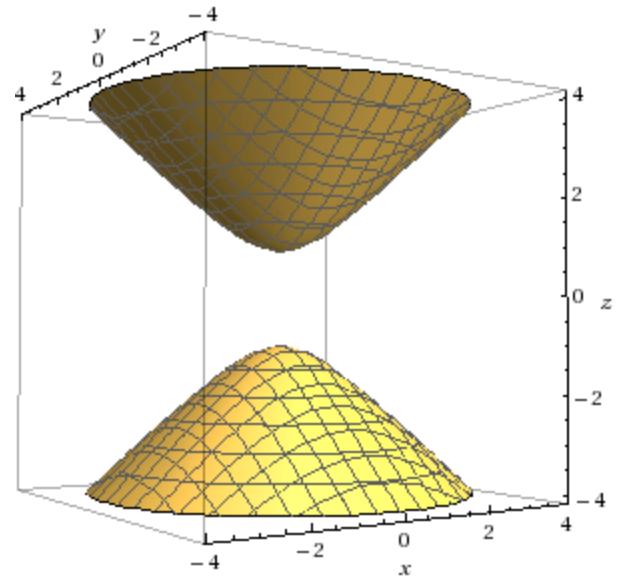
\includegraphics[scale=.13]{image/week-02-01}
	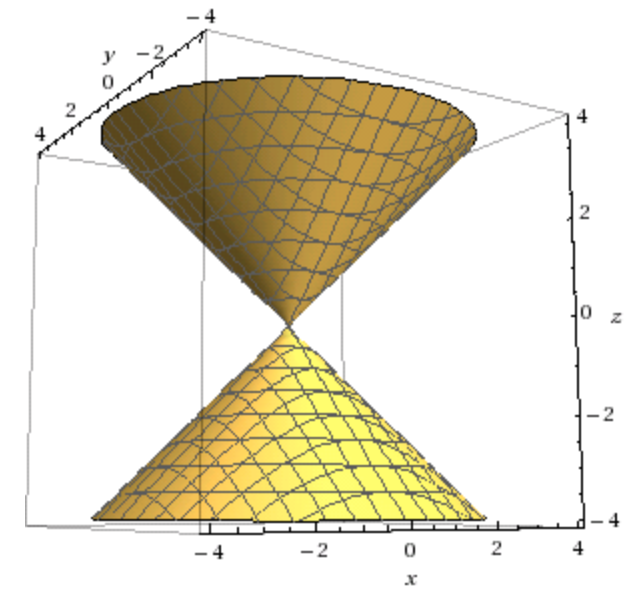
\includegraphics[scale=.13]{image/week-02-02}
	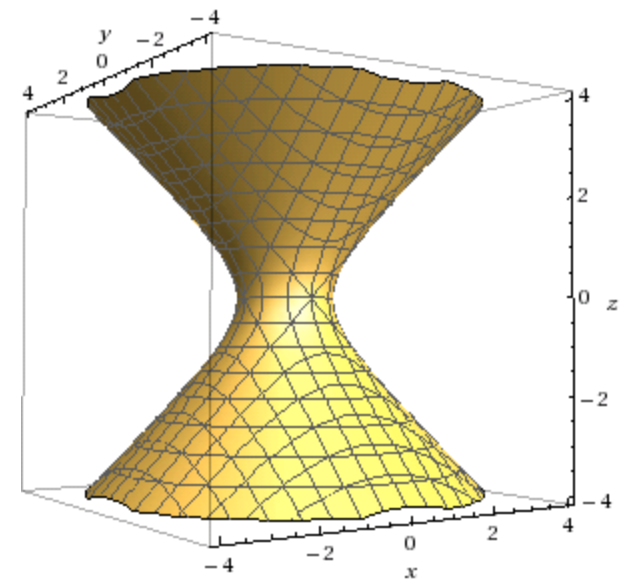
\includegraphics[scale=.13]{image/week-02-03}
	\end{center}
\end{exmp}
\end{frame}

\begin{frame}
\begin{defn}
	Let $V$ be a vector space and 
	$D$ be a open subset of $\mathbf R^n$.
	A \textbf{vector field} $\mathbf F:D\to V$ 
	is a function which assigns each point 
	$(x_1,\cdots,x_n)\in D$ a vector
	$\mathbf F(x_1,x_2,\cdots,x_n) \in V$.
\end{defn}
\begin{defn}
	Let $v,w$ be vector spaces. 
	A function $t:v\to w$ is called a 
	\textbf{linear transformation} 
	if it satisfies the following.
	\begin{enumerate}
		\item $t(v_1+v_2)=t(v_1)+t(v_2)$ 
		for all $v_1,v_2\in v$.
		\item $t(cv)= ct(v)$ for all $v\in v$ 
		and $c\in\mathbf R$.
	\end{enumerate}
\end{defn}
\begin{exmp}
	Every linear transformation can be represented by
	a matrix, and the composition of two linear
	transformation is represented by the multiplication
	of corresponding matrices.
\end{exmp}
\end{frame}



\begin{frame}
\begin{defn}\label{defn-lim-con}
	Let $f(x,y)$ be a two-variable function
	defined on the entire plane $\mathbf R^2$.
	A constant $L$ is called the 
	\textbf{limit of $f$ at $(x_0,y_0)$} if
	for any (arbitrary small) $\epsilon>0$, 
	there exists a (small) $\delta>0$
	such that whenever the distance between $(x,y)$ and $(x_0,y_0)$ is less than $\delta$,
	the inequality
	\[|f(x,y)-L|<\epsilon\]
	holds. In such case, we simply write
	\[\lim_{(x,y)\rightarrow(x_0,y_0)}f(x,y)=L\]
\end{defn}
\end{frame}

\begin{frame}
\begin{defn}
	We say a function $f(x,y)$ is 
	\textbf{continuous at $(x_0,y_0)$} if
	$$\lim_{(x,y)\rightarrow(x_0,y_0)}f(x,y)
	= f(x_0,y_0)$$
\end{defn}
\end{frame}

\begin{frame}
\begin{rem}
We say $f(x)$ is continuous at $x_0$ if	
$\lim_{x\to x_0}f(x) = f(x_0)$.
The limit $\displaystyle\lim_{x\to x_0}$ 
assumes that both right and left limits exists 
and equals to each other.
Since there are only two paths approaching $x_0$ 
in one-dimensional space, $\mathbf R$, 
the concept of the limit is intuitively clear.\\
On a two-dimensional plane, there are infinitely many directions 
and passes for $(x,y)$ to approach the limit point $(x_0,y_0)$.
The limit exists only when the limit coincides regardless
of the choice of passes (and direction) of points approaching
the limit point. This is why we need a rigorous definition of limit 
for the multivariable function.
\end{rem}
\end{frame}

\begin{frame}
\begin{exmp}
	Show that 
	\begin{equation}\label{eqn-exmp-conti}
	f(x,y)=\begin{dcases}
	\frac{xy}{\sqrt{x^2+y^2}} & (x,y)\neq(0,0)\\
	0 & (x,y)=(0,0)\end{dcases}
	\end{equation}
	is continuous at $(0,0)$.
\end{exmp}
\end{frame}

\begin{frame}
\begin{prop}
	A function $f(x,y)$ is \underline{not} 
	continuous at $(x_0,y_0)$
	if there is a path $c(t)=(x(t),y(t))$ 
	which converges to $(x_0,y_0)$ while
	$f\circ c(t)$ does not converges to $f(x_0,y_0)$.
\end{prop}
\begin{exmp}
	Let us prove that the function
	$$f(x,y)=\begin{dcases}
	\frac{x^4-4y^2}{x^2+2y^2} & (x,y)\neq(0,0)\\
	0 & (x,y)=(0,0)\end{dcases}$$
	is not continuous at $(0,0)$.
	Draw the graph and explain 
	the discontinuity on the graph.
\end{exmp}
\end{frame}

\begin{frame}
Let us explore the geometric meaning of limit (and continuity) of multi-variable function. \\
\*\newline
Suppose a function $f:\mathbb R^n\to\mathbb R^m$ satisfies $\displaystyle\lim_{\mathbf x\to\mathbf a}f(\mathbf x)=\mathbf L$. Here, the value $\mathbf L$ is a point in $\mathbb R^m$ and $\mathbf a\in\mathbb R^n$. The definition of the limit tells us that for any (small) $\varepsilon>0$, we can choose (sufficiently small) $\delta>0$ so that as long as $\mathbf x$ lies in the ball $B_\delta(\mathbf a)$ of radius $\delta$ centered at $\mathbf a$, the value $f(\mathbf x)$ lies in the ball $B_\varepsilon(\mathbf L)$ of radius $\varepsilon$ centered at $\mathbf L$. This implies that $f(B_\delta)\subset B_\varepsilon$.\\
\*\newline
In Topology, we say that a function has a limit $\mathbb L$ at $\mathbf a$ 
if however small \emph{neighborhood} $V$ of $\mathbf L$ we choose, we can always find a (very small) \emph{neighborhood} $U$ of $\mathbf a$ whose image $f(U)$ is completely contained in $V$.
\end{frame}

\begin{frame}
\begin{defn}
	Let $f(x,y)$ be a function defined on 
	a region $D\subset\mathbf R^2$ and $(x_0,y_0)\in D$. 
	Let $\mathbf u=(a,b)$ a \emph{unit} vector. 
	If the limit
	$$D_{\mathbf u}f(x_0,y_0)
	= \lim_{t\rightarrow0}\frac{f(x_0+at,y_0+bt)
	- f(x_0,y_0)}{t}$$
	exists, then it is called 
	the \textbf{$\mathbf u$-directional derivative} 
	of $f$ at $(x_0,y_0)$.
\end{defn}
\end{frame}

\begin{frame}
\begin{exmp}
	Let $f(x,y)=x^2+y^2$. 
	The $(1,0)$-directional derivative of $f$ 
	at $(\frac{1}{2},0)$ is
	\begin{align*}
	D_{(1,0)}f\left(\tfrac{1}{2},0\right)
	 &=\lim_{t\rightarrow0}\frac{f(\frac{1}{2}+t,0)
	 	- f(\frac{1}{2},0)}{t}\\
	 &=\lim_{t\rightarrow0}\frac{\left(\frac{1}{2}
	 	+ t\right)^2-(\frac{1}{2})^2}{t}=1
	\end{align*}
\end{exmp}
\end{frame}

\begin{frame}
\begin{rem}
For a single-variable function $y=f(x)$, 
the differential $f'(x_0)$ represents rate of change of 
$f(x)$ as $x$ approaches to $x$.
The directional derivative extends this concept.
Let $c(t) = (x_0,y_0) + t\mathbf u$.
$c(t)$ approaches to $(x_0,y_0)$ as $t\to 0$. 
The composition $f\circ c(t)$ is a single-variable 
function. The differential $(f\circ c)'(0)$ is
	\[(f\circ c)'(0)=D_{\mathbf u}f(x_0,y_0)\]

The directional derivative is the 
\emph{rate of chage of $f$ along straight line 
passing through $(x_0,y_0)$ 
parallel to $\mathbf u=(u_1,u_2)$}. 
Let $P$ be the plane parallel to both 
$(u_1,u_2,0)$ and $\mathbf k$ containing 
the point $(x_0,y_0,0)$.
Then $D_{\mathbf u}f(x_0,y_0)$ is the slope of 
the intersection curve between the graph of $f$ 
and the plane $P$. 
\end{rem}
\end{frame}

\begin{frame}
\begin{rem}
$f:U\to\mathbf R$ be a two-variable function
defined on a region $U\subset\mathbb R^2$.
Let $\mathbf u,\mathbf v$ be $2$-dimensional vectors.
Suppose that the $D_{\mathbf u}f(x,y)$ exists 
for all $(x,y)$ in a region $U$. 
Then we can define a new function $g$ on $U$ as
	\[g(x,y)=D_{\mathbf u}f(x,y).\]
Suppose that $g(x,y)$ has 
$\mathbf v$-direnctional derivative 
$D_{\mathbf v}g(x_0,y_0)$.
We call this as the \emph{second} directional derivative
of $f$. That is,
	$$D_{\mathbf v}D_{\mathbf u}f(x_0,y_0)
	 = D_{\mathbf v}g(x_0,y_0).$$
The value $D_{\mathbf u}f$ is the slope of the graph of 
$f$ along the $\mathbf u$-direction. 
Thus there is a unique vector tagent to the graph of $f$ 
at $(x_0,y_0,f(x_0,y_0))$ whose projection onto 
$\mathbf R^2$ is parallel to $\mathbf u$.
The value $D_{\mathbf v}D_{\mathbf u}f$ measures
how much such tangent vector \emph{changes}
along $v$-direction at $(x_0,y_0)$.\\
\*\newline
For example, $D_{\mathbf u}D_{\mathbf u}f$ 
is the acceleration $f$ in the $\mathbf u$-direction.
\end{rem}
\end{frame}

\begin{frame}
\begin{exmp}
	Let $f(x,y)=x^3+5x^2y+y^3$ 
	and $\mathbf u=(\frac{3}{5},\frac{4}{5})$.
	Find $D_{\mathbf u}f$ and 
	$D_{\mathbf u}D_{\mathbf u} f$.
\end{exmp}
\end{frame}

\begin{frame}	
\begin{defn}
	Let $\mathbf e_1=(1,0)$ and $\mathbf e_2=(0,1)$ 
	be the orthonormal vectors in $\mathbf R^2$.
	We denote $D_x$, $D_y$ for the 
	$\mathbf e_1$, $\mathbf e_2$-directional derivatives
	with respectively.
	The $D_xf(x_0,y_0)$, $D_yf(x_0,y_0)$ are called 
	the \textbf{partial derivatives} of $f(x,y)$ 
	at $(x_0,y_0)$.
	Conventionally, the partial derivatives are 
	denoted by
	$$D_xf(x_0,y_0) = f_x(x_0,y_0)
	 = \frac{\partial f}{\partial x}(x_0,y_0)$$
	$$D_yf(x_0,y_0) = f_y(x_0,y_0)
	 = \frac{\partial f}{\partial y}(x_0,y_0)$$
	We write $\displaystyle 
	\frac{\partial f}{\partial x},
	\frac{\partial f}{\partial y}$ 
	for the partial derivatives as 
	two-variable functions.
\end{defn}
\end{frame}

\begin{frame}
The second partial derivatives are denoted as
	$$\frac{\partial^2f}{\partial x^2}
	 = f_{xx}=D_{xx}f=D_x(D_xf)$$
	$$\frac{\partial^2f}{\partial x\partial y}
	 = f_{yx}=D_{xy}f=D_x(D_yf)$$
	$$\frac{\partial^2f}{\partial y\partial x}
	 = f_{xy}=D_{yx}f=D_y(D_xf)$$
	$$\frac{\partial^2f}{\partial y^2}=f_{yy}
	 = D_{yy}f=D_y(D_yf)$$
Note that $f_{xy}$ and $f_{yx}$ are \emph{not}
the same function in general.
\end{frame}

\begin{frame}
\begin{exmp}
Let 
	$$f(x,y)=\begin{dcases}
	xy\frac{x^2-y^2}{x^2+y^2}&(x,y)\neq(0,0)\\
	0& (x,y)=(0,0)
	\end{dcases}$$
Compute $f_{xy}f(0,0)$ and $f_{yx}(0,0)$.
\end{exmp}
\end{frame}

\begin{frame}
\begin{defn}
	Let $f_x(x_0,y_0)$, $f_y(x_0,y_0)$ 
	be the partial derivatives of $f(x,y)$.
	Then the function
	$$L(x,y) = f(x_0,y_0) + f_x(x_0,y_0)(x-x_0)
		+ f_y(x_0,y_0)(y-y_0)$$
	is called the \textbf{linear approximation} of 
	$f(x,y)$ at $(x_0,y_0)$.
\end{defn}
\begin{rem}
	The graph of $z=L(x,y)$ is the tangent plane
	to the graph of $z=f(x,y)$.
\end{rem}
\end{frame}

\begin{frame}
\begin{defn}
	Let $L(x,y)$ be the linear approximation of 
	$f(x,y)$ at $(x_0,y_0)$.
	We say the function $f(x,y)$ is 
	\textbf{differentiable} at $(x_0,y_0)$ if 
	the following holds.
	$$\lim_{(x,y)\rightarrow(x_0,y_0)}
	\frac{|f(x,y)-L(x,y)|}{\sqrt{(x-x_0)^2+(y-y_0)^2}}
	 = 0$$
\end{defn}
\end{frame}

\begin{frame}
\begin{exmp}
The existence of the linear approximation $L(x,y)$ 
does not imply that $f(x,y)$ is differentiable.
Find an example of a function $f(x,y)$ 
which has the linear approximation at $(0,0)$,
but not differentiable at $(0,0)$.
\end{exmp}

\begin{exmp}
Show that the function
	$$f(x,y)=\begin{dcases}
	\frac{xy}{\sqrt{x^2+y^2}} & (x,y)\neq(0,0) \\
	0 & (x,y)=(0,0)
	\end{dcases}$$
is not differentiable at $(0,0)$. 
\end{exmp}
\end{frame}

\begin{frame}
\begin{rem}
Recall that we defined the differentiability of 
single variable function as
\[\lim_{x\to x_0}\frac{f(x)-f(x_0)}{x-x_0} = f'(x_0)\]
By taking $f'(x_0)$ to the left-hand side, 
equation becomes
$$\lim_{x\to x_0}\frac{f(x)-f(x_0)
 - f'(x_0)(x-x_0)}{x-x_0} = 0$$
which is the special case of the previous definition.
\end{rem}
\end{frame}

\begin{frame}
\begin{thm}\label{thm-diff-eps}
Suppose that there are two function $\epsilon_1=\epsilon_1(x,y)$, $\epsilon_2=\epsilon_2(x,y)$ satisfying
	\begin{align*}
	f(x,y)&-f(x_0,y_0)=f_x(x_0,y_0)(x-x_0)\\
	&+f_y(x_0,y_0)(y-y_0)+\epsilon_1(x-x_0)+\epsilon_2(y-y_0).
	\end{align*}
If $\epsilon_1,\epsilon_2\rightarrow0$ as $(x,y)\rightarrow(x_0,y_0)$,
then $f(x,y)$ is differentiable at $(x_0,y_0)$.
\end{thm}
\end{frame}

\begin{frame}
\begin{defn}
Let $f:\mathbf R^n\to\mathbf R$ be a real-valued function.
The coordinates for the point $\mathbf x\in \mathbf R^n$ is denoted by 
\[\mathbf x = (x^{0}, \ldots, x^{n-1}).\]
The \textbf{gradient} of $f$ at $\mathbf x$ is the vector defined by
	\[ \nabla f = (f_{x^{0}}, \ldots, f_{x^{n-1}}) \]
Let us consider the gradient as a $n\times 1$ matrix
and the point $\mathbf x$ as a $1\times n$ matrix.
Then we say $f$ is \textbf{differentiable at} $\mathbf x_0\in\mathbf R^n$ if 
\[\lim_{\mathbf x\to\mathbf x_0}
	\frac{f(\mathbf x) - f(\mathbf x_0) 
	- \nabla f(\mathbf x_0)
	\cdot(\mathbf x-\mathbf x_0)}
	{\Vert\mathbf x-\mathbf x_0\Vert} = 0.\]
\end{defn}
\end{frame}

\begin{frame}
\begin{defn}
Let $\mathbf f:\mathbf R^n\to\mathbf R^m$ be a function
\[f(\mathbf x) = (f^{0}(\mathbf x), \ldots, f^{n-1}(\mathbf x))\]
whose coordinate functions $f^i$ are differentiable.
We call The differential of $f$ at $x_0$ is the matrix
	\[\mathbf{Df}(\mathbf x_0)
	 = \begin{bmatrix} 
	\frac{\partial f_1}{x_1}(\mathbf x_0) & \cdots 
		& \frac{\partial f_1}{x_n}(\mathbf x_0) \\
	\vdots & \ddots & \vdots \\
	\frac{\partial f_m}{x_1}(\mathbf x_0) & \cdots
		& \frac{\partial f_m}{x_n}(\mathbf x_0) 
	   \end{bmatrix}\]
	Then $f$ is differentiable at $\mathbf x_0$ if
	$$\lim_{\mathbf x\to\mathbf x_0}
	\frac{f(\mathbf x) - f(\mathbf x_0) 
	- Df(\mathbf x_0)
	(\mathbf x - \mathbf x_0)}
	{\Vert \mathbf x - \mathbf x_0\Vert} = \vec 0$$
\end{defn}	
\end{frame}

\begin{frame}
\begin{prob}
	Draw the graph of 
	\begin{enumerate}
	\item $z = x(x^2-y^2)$ 
	(This surface is called Monkey's saddle.)
	\item $f(x,y)=\begin{dcases}
	\frac{xy}{\sqrt{x^2+y^2}} & (x,y)\neq(0,0)\\
	0 & (x,y)=(0,0)\end{dcases}$
	\end{enumerate}
\end{prob}
\end{frame}

\begin{frame}
\begin{prob}
	Show that 
	\[\lim_{(x,y)\to(0,0)} \frac{|xy|}{x^2+y^2}\]
	does not exist.
\end{prob}
\end{frame}

\begin{frame}
\begin{prob}
	Show that the function
	$$f(x,y)=\begin{dcases}
	\frac{y^2}{|x-y|} & x\neq y\\
	0 & x=y\end{dcases}$$
	is discontinuous at $(0,0)$.
\end{prob}	
\end{frame}

\begin{frame}
\begin{prob}
	Consider the following statements.
	\begin{enumerate}
		\item The partial derivatives $f_x,f_y$ are continuous at $(x_0,y_0)$.
		\item The function $f$ is differentiable at $(x_0,y_0)$.
		\item The directional derivative $D_{\mathbf u}f(x_0,y_0)$ exists for every $\mathbf u$.
		\item The function $f$ is continuous at $(x_0,y_0)$.
	\end{enumerate}
	Show that the following implications hold.
	\begin{itemize}
		\item $1\Rightarrow 2$
		\item $2\Rightarrow 3$
		\item $2\Rightarrow 4$
	\end{itemize}
	Find the counter-examples for 
	\begin{itemize}
		\item $2\Rightarrow 1$
		\item $3\Rightarrow 2$
		\item $4\Rightarrow 2$
	\end{itemize}
\end{prob}	
\end{frame}
\end{document}